\Subsection{Билет 69: Два доказательства теоремы Коши о дифференциальной форме $f(z) \,dz$}

\begin{designations}
	$f\in H(\Omega)$ означает, что $f:\Omega \to \CC$ и голоморфна во всех точках
\end{designations}

\begin{theorem}[Коши]\thmslashn
	
	$f\in H(\Omega) \Rightarrow f(z)\,dz$ -- локально точная функция
	
\end{theorem}

\begin{proof}\thmslashn

	\begin{enumerate}
		\item 
		Для случая, когда $\frac{\partial f}{\partial x}$ и $\frac{\partial f}{\partial y}$ непрерывны
		
		$f(z)dz$ -- замкнутая форма
		
		$f(z)dz = (g(z) + ih(z))(dx + idy) = (g(z)dx - h(z)dy) + i(h(z)dx + g(z)dy)$
		
		$
		\begin{aligned}
		\frac{\partial g}{\partial x} &= \frac{\partial h}{\partial y} \Rightarrow hdx + gdy\text{ -- замкнута}\\
		\frac{\partial g}{\partial y} &= -\frac{\partial h}{\partial x} \Rightarrow gdx - hdy\text{ -- замкнута}
		\end{aligned} \Rightarrow f$ замкнута $\Rightarrow$ $fdz$ локально точна
	
		\item
		Для произвольного случая
		
		Рассмотрим какой-нибудь круг, содержащийся в $\Omega$ 
		
		Нам надо проверить что в этом круге есть первообразная $\Rightarrow$ надо проверить, что $\int$ по любому прямоугольнику из этого круга равен нулю $\alpha(P) = \int\limits_{P} f(z)\,dz$ 
		
		Допустим, что это не $0$
		
		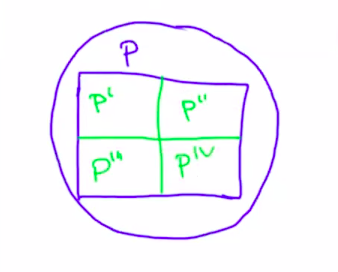
\includegraphics[scale=0.5]{pic_1}
		
		$\alpha(P) = \alpha(P') + \alpha(P'') + \alpha(P''') + \alpha(P'''')$ 
		
		$\abs{\alpha(P)} \leqslant \abs{\alpha(P')} + \abs{\alpha(P'')} + \abs{\alpha(P''')} + \abs{\alpha(P'''')}$
		
		Пусть $P_1$ -- такой прямоугольник, что $\abs{\alpha(P_1)} \geqslant \frac{1}{4}\abs{\alpha(P)}$
		
		Пусть $P_2$ -- такая четвертинка $P_1$, что $\abs{\alpha(P_2)} \geqslant \frac{1}{4^2}\abs{\alpha(P)}$ и т.д. $\abs{\alpha(P_k)} \geqslant \frac{1}{4^k}\abs{\alpha(P)}$
		
		$P\supset P_1 \supset P_2 \supset \ldots$ у них есть общая точка $z_0 \in \Omega$
		
		$f$ голоморфна в точке $z_0 \Rightarrow f(z) = f(z_0) + f'(z_0)(z - z_0) + \varepsilon (z-z_0)|z-z_0|$
		
		$\int\limits_{P_n} f(z)\,dz = \int\limits_{P_n} f(z_0)\,dz + \int\limits_{P_n} f'(z_0)(z- z_0)\,dz + \int\limits_{P_n} \varepsilon (z-z_0)|z-z_0|\,dz$
		
		$\int\limits_{P_n} f(z_0)\,dz = 0 = \int\limits_{P_n} f'(z_0)(z- z_0)\,dz$ 
		
		Оценим оставшийся 3 интеграл
		
		$\abs{\int\limits_{P_n} \varepsilon (z-z_0)|z-z_0|\,dz} \leqslant \left(\text{периметр} P_n\right)^2 \max\abs{\varepsilon(z-z_0)} = \frac{1}{4^n}\left(\text{периметр} P\right)^2 \max\abs{\varepsilon(z-z_0)} \Rightarrow 0 < \frac{|\alpha(P)|}{\left(\text{периметр} P\right)^2}\leqslant \max\abs{\varepsilon(z-z_0)}$
		
		Противоречие, т.к. правая часть может быть сколь угодно маленькой, а левая часть константа
	\end{enumerate}

\end{proof}
